
\hypertarget{cv:registrarPostcondicion}{\section{Registrar Postcondición}} \label{sec:registrarPostcondicion}

	Esta funcionalidad le permitirá registrar una postcondición dentro del caso de uso que se esta operando.

		\subsection{Procedimiento}

			%Pasos de procedimiento
			\begin{enumerate}
	
			\item Oprima el botón \IURegistrar{} de la pantalla \ref{fig:GestionarPostcondiciones} ''Gestionar Postcondiciones''.
			
			\item Se mostrará la pantalla \ref{fig:registrarPostcondicion} ''Registrar Postcondición''.

			%Pantalla
			\begin{figure}[htbp!]
				\begin{center}
					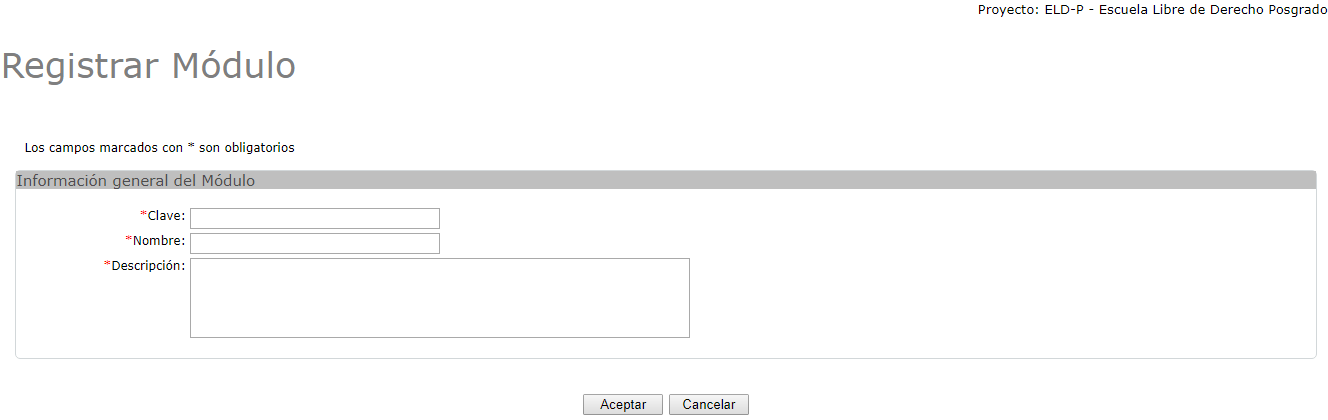
\includegraphics[scale=0.5]{roles/lider/casosUso/pantallas/IU5-1registrarModulo}
					\caption{Registrar Postcondición}
					\label{fig:registrarPostcondicion}
				\end{center}
			\end{figure}
		
			\item Ingrese la redacción de la postcondición.
			
			\item Para la redacción podrá ingresar TOKENS para vincular diferentes elementos previamente registrados:
			
			\begin{itemize}
				\item Podrá referenciar elementos de tipo actor con el TOKEN: ''ACT·''.
				\item Podrá referenciar elementos de tipo entidad y/o atributos con los TOKEN: ''ENT·''y ''ATR·''.
				\item Podrá referenciar elementos de tipo término con el TOKEN: ''GLS·''.
			\end{itemize}
			
			\item Oprima el botón \IUAceptar.
			
			\item Se mostrará el mensaje \ref{fig:postcondicionRegistrada} en la pantalla \ref{fig:GestionarPostcondiciones} ''Gestionar Postcondiciones''.
			
			\begin{figure}[htbp!]
				\begin{center}
					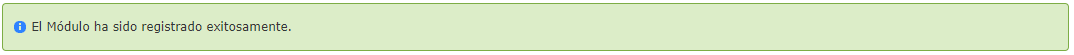
\includegraphics[scale=0.6]{roles/lider/casosUso/pantallas/IU5-1MSG1}
					\caption{MSG: Postcondición Registrada}
					\label{fig:postcondicionRegistrada}
				\end{center}
			\end{figure}
			\end{enumerate}